% ============================================================
% SECCIÓN: Compartimentalización del modelo DEB
% Desarrollo conceptual para tesis doctoral
% ============================================================

El modelo dinámico de presupuesto energético diferencial (DEB) propuesto por \textcite{eriksenDynamicModellingFeed2022} estructura la biomasa larval como un sistema termodinámico abierto: intercambia materia y energía con el ambiente (sustrato y gases de respiración) mientras conserva la identidad biológica del individuo. A diferencia de los modelos logísticos clásicos, que tratan al animal como una masa indiferenciada $W(t)$, el DEB separa explícitamente los flujos de carbono según su destino metabólico. Esta distinción es indispensable para la presente investigación porque permite predecir simultáneamente (i) la acumulación de biomasa comercial, (ii) el contenido lipídico (relevante para biodiésel y alimento) y (iii) la emisión de $\mathrm{CO_2}$, variable que se contrastará directamente contra las lecturas de los sensores NDIR del reactor batch.

\subsection{El individuo larval como sistema de tres compartimentos}

\textcite{eriksenDynamicModellingFeed2022} divide la larva en tres reservorios de carbono, cada uno con una función fisiológica bien definida (Figura~\ref{fig:compartimentos-deb}). Todas las cantidades se expresan en \textbf{equivalentes de carbono} ($\si{mg\,C}$), lo que permite sumar directamente flujos de distinta naturaleza química (carbohidratos, lípidos, proteínas) mediante una moneda metabólica común.

\begin{figure}[htbp]
    \centering
    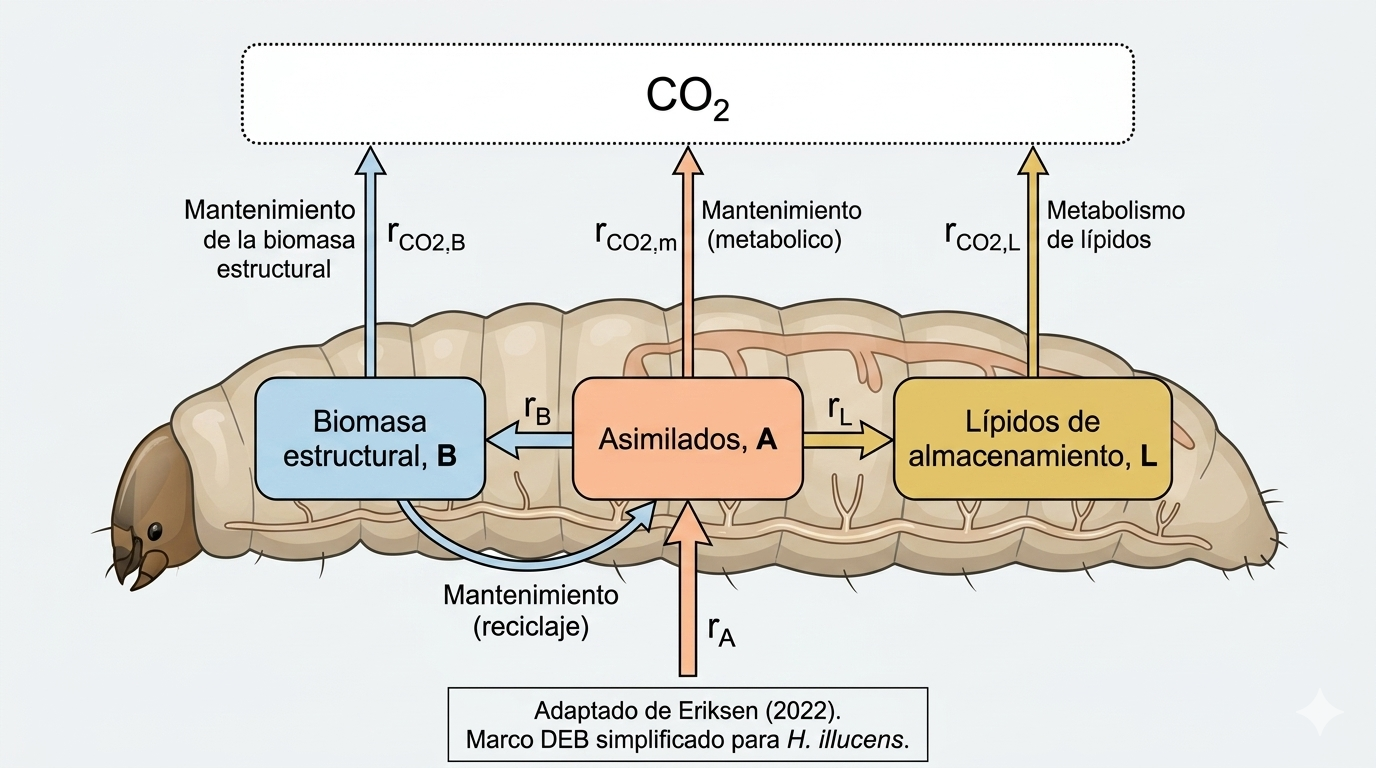
\includegraphics[width=0.95\textwidth]{00Figuras/modelo-deb}
    \caption{Esquema de compartimentos del modelo DEB de \textcite{eriksenDynamicModellingFeed2022} para \textit{Hermetia illucens}. El sustrato orgánico se asimila en el pool $A$, desde donde el carbono fluye hacia biomasa estructural $B$, lípidos de almacenamiento $L$ o se pierde como $\mathrm{CO_2}$ por respiración. El pool $A$ opera en estado estacionario ($\mathrm{d}A/\mathrm{d}t=0$).}
    \label{fig:compartimentos-deb}
\end{figure}

\subsubsection{Pool de asimilados $A$}

El compartimento $A$ representa el conjunto de moléculas que han sido absorbidas a través de la pared intestinal y liberadas a la hemolinfa, pero que aún no han sido incorporadas a tejidos permanentes ni oxidadas para generar energía. Incluye azúcares, aminoácidos, ácidos grasos y metabolitos intermediarios en tránsito.

\textbf{Hipótesis de estado estacionario.} \textcite{eriksenDynamicModellingFeed2022} asume que la masa de $A$ es despreciable frente a $B$ y $L$, y que el pool se vacía instantáneamente:
\begin{equation}
    \frac{\mathrm{d}A}{\mathrm{d}t} = 0.
    \label{eq:dA_dt}
\end{equation}
Esta simplificación tiene dos justificaciones biológicas. Primera, en insectos holometábolos con alto metabolismo, el tiempo de tránsito intestinal es del orden de minutos a horas, mientras que el ciclo larval completo dura semanas; por tanto, el retardo entre ingestión y asignación es negligible en la escala de tiempo del modelo. Segunda, el pool $A$ no es medible experimentalmente con las técnicas estándar (peso seco, extracción lipídica, análisis elemental), de modo que tratarlo como variable dinámica introduciría un parámetro no observable y no identificable.

Desde el punto de vista algebraico, la condición $\mathrm{d}A/\mathrm{d}t=0$ convierte a $A$ en un \emph{nodo de Kirchhoff}: la tasa de entrada $r_A$ se distribuye instantáneamente entre las tasas de salida $r_B$, $r_L$ y las tres vías respiratorias $r_{\mathrm{CO_2},m}$, $r_{\mathrm{CO_2},B}$, $r_{\mathrm{CO_2},L}$.

\subsubsection{Biomasa estructural $B$}

La biomasa estructural agrupa todo el tejido que mantiene la integridad morfológica y funcional de la larva: músculos, tegumento (exoesqueleto quitinoso), tracto digestivo, sistema nervioso y órganos internos. Excluye \emph{deliberadamente} a los lípidos de reserva, que se contabilizan en $L$.

\textbf{¿Por qué separar $B$ de $L$?} En \textit{H.~illucens} la composición bioquímica cambia drásticamente con la edad. Las larvas neonatas poseen aproximadamente $\SI{10}{\percent}$ de lípidos en peso seco, mientras que las prepupas bien alimentadas alcanzan hasta $\SI{47}{\percent}$ \parencite{eriksenDynamicModellingFeed2022}. Si el modelo usara una sola variable de peso total, esta variabilidad quedaría oculta. Al separar $B$ (relativamente constante en composición) de $L$ (altamente variable), el modelo puede predecir:
\begin{itemize}
    \item El peso seco comercial $X_{\mathrm{DW}}$ (suma de $B$ y $L$ convertidos a masa seca).
    \item El rendimiento lipídico, crítico para la valorización económica del bioproducto.
    \item El momento óptimo de cosecha, cuando la relación $L/B$ es máxima para biodiésel o mínima para proteína animal.
\end{itemize}

La ecuación de balance para $B$ es directa:
\begin{equation}
    \frac{\mathrm{d}B}{\mathrm{d}t} = r_B,
    \label{eq:dB_dt}
\end{equation}
donde $r_B$ es la tasa neta de síntesis de tejido estructural, expresada en $\si{mg\,C\,dia^{-1}}$.

\textbf{Nota sobre lípidos estructurales.} Aunque $B$ excluye a los lípidos de reserva, sí contiene una fracción intrínseca de lípidos membranales y de señalización (fósfolípidos, esfingolípidos) que no se movilizan durante el ayuno. Esta fracción se denota $\delta_{L,B}=\num{0.10}$ y se suma al total medible:
\begin{equation}
    L_{\mathrm{tot}} = L + \delta_{L,B}\,B.
    \label{eq:L_tot}
\end{equation}
Así, $L_{\mathrm{tot}}$ representa lo que un laboratorio reportaría como ``contenido lipídico'' tras extracción con solventes, mientras que $L$ es la reserva metabólicamente activa.

\subsubsection{Lípidos de almacenamiento $L$}

El compartimento $L$ modela el cuerpo graso (fat body) de la larva: triacilgliceroles almacenados en adipocitos que sirven como reserva energética de largo plazo. Su dinámica es la más flexible del sistema:
\begin{itemize}
    \item \textbf{Acumulación} ($r_L > 0$): cuando la asimilación supera las necesidades de mantenimiento y crecimiento estructural, el excedente se esterifica y almacena.
    \item \textbf{Reciclaje} ($r_L < 0$): cuando el sustrato escasea o la larva entra en prepupa, los lípidos se hidrolizan y devuelven carbono al pool $A$ para mantenimiento.
\end{itemize}

El balance incluye el aporte de lípidos estructurales que acompañan al crecimiento de $B$:
\begin{equation}
    \frac{\mathrm{d}L_{\mathrm{tot}}}{\mathrm{d}t} = r_L + \delta_{L,B}\,r_B.
    \label{eq:dLtot_dt}
\end{equation}
El término $\delta_{L,B}\,r_B$ indica que cada miligramo de carbono nuevo en biomasa estructural arrastra consigo $\num{0.10}\,\si{mg\,C}$ de lípidos membranales indispensables.

\subsection{Unidades y moneda metabólica}

El uso de equivalentes de carbono como unidad base tiene ventajas metodológicas para esta investigación:
\begin{enumerate}
    \item \textbf{Aditividad.} Un $\si{mg\,C}$ de carbohidrato, uno de proteína y uno de lípido suman $3\,\si{mg\,C}$ de flujo total, independientemente de su estado redox.
    \item \textbf{Conversión directa a $\mathrm{CO_2}$.} La respiración se calcula como masa de carbono oxidado; la conversión a volumen de gas en el batch cerrado solo requiere la masa molar de $\mathrm{CO_2}$ ($M_{\mathrm{CO_2}}=\SI{44.01}{g\,mol^{-1}}$) y las condiciones de presión y temperatura del reactor.
    \item \textbf{Compatibilidad con análisis elemental.} Los datos experimentales de contenido de carbono (analizador CHN) se insertan directamente sin factores de conversión empíricos.
\end{enumerate}

Las conversiones a peso seco ($X_{\mathrm{DW}}$) y peso húmedo ($X_{\mathrm{WW}}$) se realizan al final de la simulación mediante los factores de conversión de la Tabla~\ref{tab:parametros-conversion}, permitiendo comparar las predicciones del modelo con las mediciones gravimétricas del laboratorio.

\begin{table}[htbp]
    \centering
    \caption{Factores de conversión y parámetros cinéticos del modelo DEB de \textcite{eriksenDynamicModellingFeed2022} para \textit{Hermetia illucens} en sustrato pollo, condiciones óptimas.}
    \label{tab:parametros-conversion}
    \begin{tabular}{@{}llcl@{}}
        \toprule
        \textbf{Símbolo} & \textbf{Descripción} & \textbf{Valor} & \textbf{Fuente} \\
        \midrule
        \multicolumn{4}{@{}l}{\textit{Parámetros de conversión}} \\
        $\delta_{C,B}$ & Fracción de carbono en biomasa estructural orgánica & \num{0.49} & \textcite{roels1980} \\
        $\delta_{C,L}$ & Fracción de carbono en lípidos (base: trilaurina) & \num{0.79} & \textcite{eriksenDynamicModellingFeed2022} \\
        $\delta_{L,B}$ & Fracción de lípidos intrínsecos en biomasa estructural & \num{0.10} & Fig.~2C, \textcite{eriksenDynamicModellingFeed2022} \\
        $\delta_{O}$ & Fracción orgánica del peso seco total & \num{0.90} & Mediana literatura$^{\text{a}}$ \\
        $\delta_{\mathrm{DW},B}$ & Fracción de peso seco en biomasa estructural húmeda & \num{0.25} & Fig.~2D, \textcite{eriksenDynamicModellingFeed2022} \\
        $\delta_{I}$ & Ratio de peso entre mudas sucesivas & \num{5} & \textcite{jucker2017, macavei2020} \\
        \midrule
        \multicolumn{4}{@{}l}{\textit{Parámetros cinéticos (sustrato pollo)}} \\
        $a_{\max}$ & Tasa específica máxima de asimilación & \SI{1.4}{\per\day} & Ajuste Fig.~3A, \textcite{eriksenDynamicModellingFeed2022} \\
        $m$ & Tasa específica de mantenimiento & \SI{0.08}{\per\day} & \textcite{eriksenDynamicModellingFeed2022} \\
        $Y_{B}$ & Costo de síntesis de biomasa estructural & \num{0.44} & \textcite{eriksenDynamicModellingFeed2022} \\
        $Y_{L}$ & Costo de síntesis de lípidos de almacenamiento & \num{0.42} & \textcite{kok2021} \\
        $\alpha$ & Coeficiente de reducción logística de asimilación (instar 6) & \num{0.92} & Ajuste Fig.~3A, \textcite{eriksenDynamicModellingFeed2022} \\
        $\beta$ & Coeficiente de reducción logística de crecimiento estructural & \num{2.02} & Ajuste Fig.~3A, \textcite{eriksenDynamicModellingFeed2022} \\
        $B_{\max,0}$ & Biomasa estructural máxima (condiciones óptimas) & \SI{65}{\milli\gram\,C} & Ajuste Fig.~3A, \textcite{eriksenDynamicModellingFeed2022} \\
        $t_{p,\min}$ & Tiempo mínimo de desarrollo (neonata a prepupa) & \SI{13}{\day} & \textcite{chia2018}$^{\text{b}}$ \\
        $\rho$ & Tasa de decrecimiento de $B_{\max}$ tras $t_{p,\min}$ & \SI{1}{\milli\gram\,C\,\per\day} & Ajuste, \textcite{eriksenDynamicModellingFeed2022} \\
        \bottomrule
    \end{tabular}
    \begin{flushleft}
        \footnotesize $^{\text{a}}$Mediana de 10 estudios independientes \parencite{eriksenDynamicModellingFeed2022}.\\
        \footnotesize $^{\text{b}}$Valor umbral reportado para condiciones de laboratorio óptimas.
    \end{flushleft}
\end{table}
